\chapter{DNS}
\label{chap:dns}

DNS bietet ein Service zur standardisierten Auflösung von Ressourcennamen innerhalb globaler oder lokaler Computernetzwerke \cite{rfc1035}. Dabei werden menschenlesbare Zeichenketten (Namen) in Adressen übersetzt. Des Weiteren ist es möglich zusätzliche Informationen über diese Namen vom System abzufragen.

\section{Aufbau des DNS}

DNS ist als globale Datenbank mit Baum-Struktur konzipiert, welche über eine beliebige Anzahl an vernetzten Rechnern verteilt wird. Der Wurzelknoten der Baums wird dabei als Root bezeichnet und von der Internet Assigned Numbers Authority (IANA), kontrolliert durch ein Komitee der \textit{Internet Corporation for Assigned Names and Numbers} (ICANN), verwaltet. Die Daten dieses Root-Knotens werden über 13 global verteilte Server bereitgestellt. 
Knoten der darunterliegenden und damit ersten Ebene werden als \textit{Top Level Domains} (TLDs) bezeichnet und sind nach Ländern (country-code TLD; ccTLD) oder Verwendung (genric TLD; gTLD) gruppiert. Da mache Funktionen von DNS spezielle Domänen benötigen, existiert eine spezielle Infrastruktur-TLD (.arpa) die direkt von IANA/ICANN verwaltet wird. Die anderen TLDs werden von verschiedenen Institutionen betrieben und stellen die höchste Stelle der DNS-Hierarchie dar. Diese sind für die Weitergabe der Verwaltungsrechte der ihnen nachfolgende Unterdomänen (Subdomains), sogenannte Second Level Domains (SLDs), verantwortlich. Die TLD .com wird, als Beispiel, von Verisign, Inc. betreut. Versign tritt somit als \textit{Registrar} der TLD .com auf. Will nun eine Person das Recht zur Verwaltung einer der .com Domäne nachgefolgten SLD erhalten, muss dies über einen Antrag bei dem Registrar, sprich Verisign, erfolgen. Ist die gewünschte Domäne, z.B. example.com, noch nicht vergeben, werden die Verwaltungsberechtigungen, gegen eine Gebühr, in den Besitz der Antragstellenden übergehen. Alle untergeordneten Domänen sind damit ebenfalls in deren Verantwortung übergegangen. Dieser Aufbau führt zu einer schichtweisen Delegation der Aufgaben innerhalb des globalen DNS-Namensraums (siehe Abb. \ref{img:dnsnamespace}). 

\begin{figure}[!hb]
    \centering
    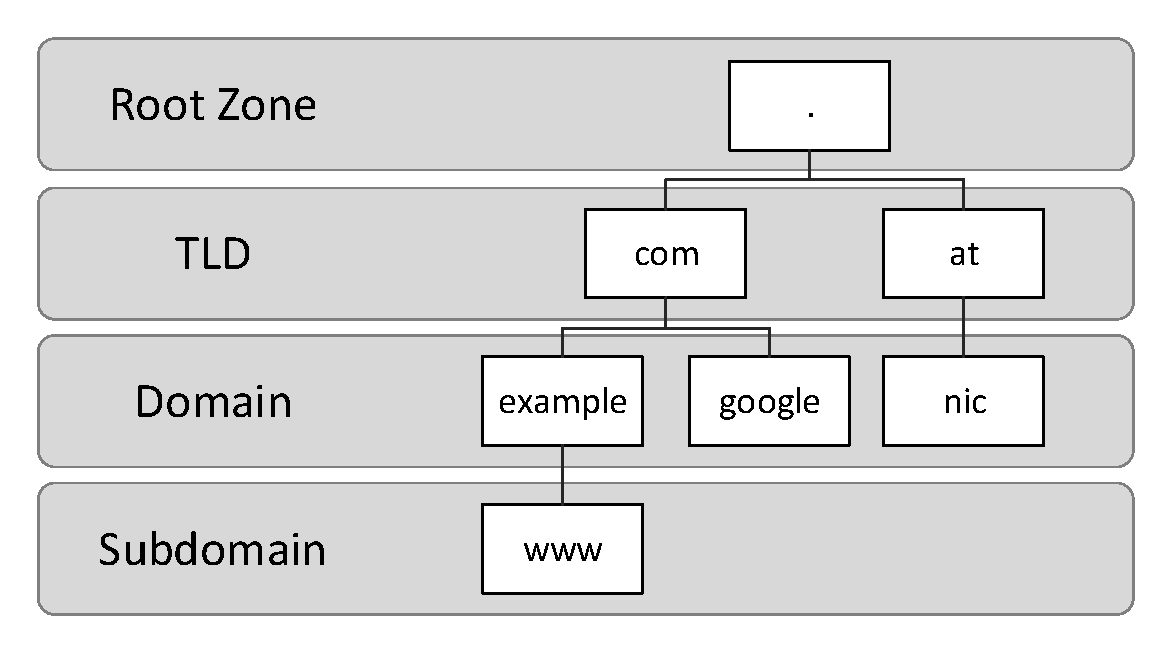
\includegraphics[width=0.5\textwidth]{DNS_NameSpaceLayers}
    \caption{Aufbau des DNS}
    \label{img:dnsnamespace}
\end{figure}

\section{Ressource Records, Sets und Zonen}

Alle Datensätze in DNS werden in einer als \textit{Ressource Record} (RR) bezeichneter Datenstruktur abgelegt. Ein RR besteht dabei aus 5 Informationen: Namen, Time-To-Live (TTL), Klasse (Class), Typ (Type), Datenfeld (Data). Dabei sind die Felder TTL und Class optional. Die Menge an Einträgen mit gleichen Werten der Felder Name, TTL, Class und Type bilden dabei ein \textit{Ressource Record Set} (RRset) \cite{rfc2181}, das kleinstmögliche abfragbare Element in DNS. Alle RR die einem definierten, zusammenhängenden Teil des DNS Namensraum zugeordnet sind, werden als Zone bezeichnet. Diese Sammlung an RR wird in einer Datei, dem \textit{Zone File}, gespeichert und von DNS-Server-Implementationen als Datenbasis genutzt.   

Wie in Listing \ref{lst:dnsZoneFile} zu sehen ist, werden die Daten in einem menschenlesbaren Format gespeichert. Zeile 1 enthält die Anweisung den Namens \texttt{test.example.com.} zu den IPv4-Adressen \texttt{172.30.0.7} und \texttt{172.30.0.8} aufzulösen. Zeile 3 fügt dem Namen weiter Information im Freitextformat hinzu. Zeile 1 und 2 bilden zusammen ein RRset für \texttt{test.example.com 3600 IN A}.

\begin{lstlisting}[caption={Ausschnitt aus dem Zone-File \textit{example.com}}, label={lst:dnsZoneFile}]
test.example.com.  3600  IN  A       172.30.0.7
                         IN  A       172.30.0.8
                         IN  TXT     "Text"
example.com.       1800  IN  MX      10 test.example.com.
example.com.       1800      NS      nameserver.example.org.
nameserver               IN  A       172.30.0.2
                         IN  AAAA    2001:db8:10::2
\end{lstlisting}

\section{DNS Server}
\label{sec:dnsserver}

Um die globale, verteilte Datenbank des DNS nutzen zu können, ist es notwendig, dass diese den DNS-Client-Programmen zugänglich gemacht wird. Das Netzwerkprotokoll ist nach dem klassischen Client-/Server-Konzept ausgestaltet. Es erfordert keinen Verbindungsaufbau und verwendet einen einfachen, sequenziellen Ablauf an Anfragen und Antworten. Ein Client stellt dabei immer nur Anfragen an Server und verarbeitet deren Antwort. DNS-Server können hingegen, je nach Typ, auch selbst Anfragen an andere Server stellen und sind somit nicht nur auf das Beantworten von Anfragen beschränkt. Es können dabei vier unterschiedliche DNS-Server-Typen festgemacht werden.

Die Software, die auf jedem Client-Rechner DNS-Anfragen von Programmen entgegennimmt und diese an die DNS Infrastruktur zur Auflösung übergibt, werden als \textbf{Stub Resolver} bezeichnet. Diese können nach außen ausschließlich mit \textit{rekursiven Resolvern} kommunizieren und nehmen selbst keine DNS-Namensauflösung vor. In manchen Fällen verfügen sie jedoch über einen Cache oder können aufgrund lokaler Policies (z.B. einem Hosts-File) eine Namensauflösung auf anderem Wege durchführen.

\textbf{Rekursive Resolver} (Recursive Resolver) sind spezielle DNS-Server die von Clients genutzt werden um Namen aufzulösen. Sie verfügen meistens über keine eigenen Zonen und sind damit als Vermittlungskomponente zwischen Endgeräten und den im Internet verfügbaren DNS-Servern zu verstehen.

Server deren Hauptaufgaben im Auflösen von Namen einer oder mehrerer bestimmter Zonen besteht, werden \textbf{authoritative Server} genannt. Die Bezeichnung spiel auf den Umstand an, dass die Antworten dieses Servers die finale Wahrheit über die von ihm verwalteten Zonen darstellt. Sie lesen die Antworten direkt auf dem Zonen-File der entsprechenden Zone und verlassen sich nicht auf Antworten anderer Server oder Caches. Authoritative DNS-Server stellen damit die Endpunkte der Auflösung für die jeweiligen Domänen dar.

Eine spezielle Form des \textit{Rekursive Resolver} wird als \textbf{Forwarding DNS Server} oder \textit{Forwarding Resolver} bezeichnet. Aus Sicht des Stub Resolvers verhält er sich wie ein gewöhnlicher Rekursiver Resolver. Der Unterschied besteht darin, dass er selbst keinen Auflöseprozess durchführt- Die Anfragen werden lediglich an einen anderen Server weiterleitet, welche die eigentliche Auflösung durchführen. Die Ergebnisse werden meist gecacht bevor sie an den Client weitergegeben werden. Dies ist der Grund warum diese Server in seltenen Fällen auch als \textit{DNS-Netzwerk-Cache} oder \textit{Cache-Only Resolver} bezeichnet werden. 

\section{DNS Namensauflösungsprozess}
\label{sec:dnsresolution}

Der Namensauflösungsprozess erfolgt über mehrere Schritte und kann am besten anhand eines Beispiels dargestellt werden. Nehmen wir an, eine Applikation möchte die IPv4-Adresse des Namen \texttt{example.com} herausfinden und stellt eine Anfrage an den lokalen Stub Resolver (kurz stub) des Client. Der Prozess in Abb. \ref{img:dnsresolution} visualisiert und kann Schrittweise wie folgt beschrieben werden:

\begin{enumerate}
    \item Der stub stellt eine Anfrage nach dem Type A Record der Domäne example.com an den für ihn konfigurierten rekursiven Resolver.
    \item Der resolver empfängt die Anfrage und prüft seinen lokalen Cache nach dem Eintrag. Da er diesen nicht aufgefunden wird fortgefahren.
    \item Nun startet der resolven den rekursiven Auflösungsvorgang. Geht man von einem leeren Cache aus, wird mit der Root-Zone (.) begonnen. Die Anfrage nach www.example.com wird dafür an einen der 13 vorkonfigurierten Root-DNS-Server gesendet.
    \item Der Root-Server empfängt die Anfrage, kann jedoch nur den TLD Teil der Antwort auflösen. Es sendet daher die Adressen des authoritativen Nameserver für die TLD .com zurück.
    \item Der Resolver verarbeitet nun die Adressen und sendet die Anfrage an einen der authoritativen Server der .com Domäne.
    \item Der TLD Nameserver empfängt die Anfrage und prüft, ob für die Domäne example.com eine entsprechende Deligation existiert. Da diese in Form mehrerer NS Einträge vorliegt, wird eine Liste an authoritativen Nameserver-Adressen der SLD Domäne example.com als Antwort gesendet.
    \item Da nun die Adresse eines authoritative Servers für die vollständige Zieldomäne example.com gefunden wurde, kann die gewünschte Information abgefragt werden. Der Resolver sendet also ein letztes mal die Anfrage des Client, jetzt an den Nameserver der SLD example.com.
    \item Der authoritative Server der SDL example.com nimmt die Anfrage nach dem RR mit Typ A für die Domäne example.com entgegen und liefert nun die gewünschte Information in Form einer IPv4 Adresse.
    \item Der rekursive Resolver empfängt die Antwort, überträgt sie in seinen Cache und sendet dem anfragenden stub die IPv4 Adresse zurück.
\end{enumerate}

\begin{figure}[htbp]
    \centering
    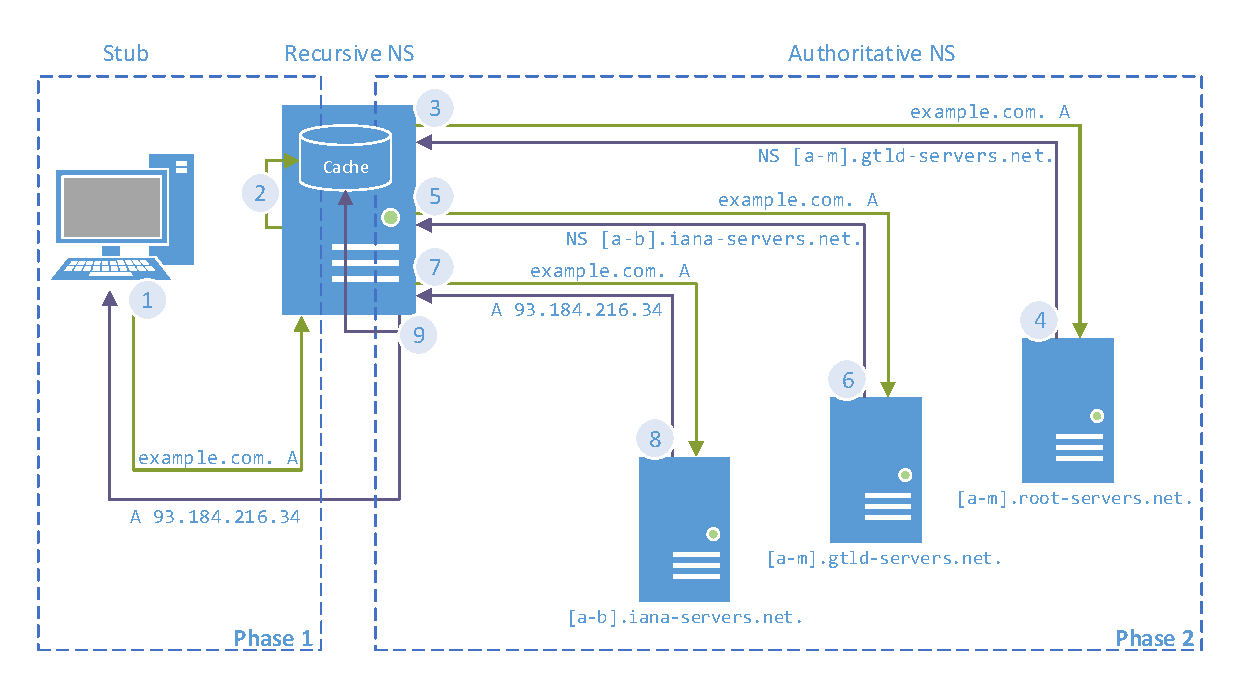
\includegraphics[width=\textwidth]{DNS_Resolution}
    \caption{Der schrittweise dargestellte Auflösungsprozess des Namen \texttt{example.com} über DNS. Der zeitliche Ablauf wird über die nummerierten Markierungen angezeigt.}
    \label{img:dnsresolution}
\end{figure}

\section{Informationssicherheit}
\todo[inline]{Definition Informationssicherheit, kurzes Bescheiben der CIA-Triade, Privacy definieren, Trust (CoT, WoT, SK, TOFU).}
\todo[inline]{Cyber-Kill-Chain erklären (Verweis unter Angriffe)}

\section{DNS Security}
\label{sec:dnssecurity}

Obwohl oder gerade weil DNS eines der grundlegendsten Services im Internet darstellt wurde bei der Spezifikation des Netzwerkprotokolls bewusst auf eine Authentifizierung verzichtet. Dies ist auf die Idee einer öffentlich zugänglichen, globalen Datenbank, nach dem Vorbild eines globalen Telefonregisters, zurückzuführen. Die Datenbasis der Namensauflösung wurde somit als frei öffentlich zugänglich definiert. Abgesehen davon, stammt das Protokoll aus einer Zeit inder modernen Schutzzielen wie Sicherheit und Vertraulichkeit wenig Beachtung geschenkt wurde. Dies führten zu einer Vernachlässigung des Sicherheitsgedanken und hat sich über die Zeit zu einem ernstzunehmenden Problem entwickelt. Verschärfend kommt hinzu, dass kein allgemeiner Konsenz über die Sicherheitsziele herrscht. Dies Erschwert die Entwicklung einer Lösung und hat zu den unterschiedlichsten Ansätzen und Technologien geführt \cite{Grothoff2018}. Die relevanten Sicherheitsziele werden in Kapitel \ref{chap:goals} näher behandelt. Sieht man von den Schwachstellen des Netzwerkprotokolls (siehe Kapitel \ref{chap:threads}) ab, gibt es einige folgende wichtige Punkte die in Betracht gezogen werden müssen um die Probleme der DNS Sicherheit zu erfassen.

\subsection{Resolver Position}
Der Aufbau der Client-nahen Infrastruktur spielt eine wichtige Rolle für die Sicherheit des Clients. Wie im Abschnitt \ref{sec:dnsresolution} beschrieben, wird vom Client einen Recursive Resolver benötigt um die eigentliche Auflösung der Namen durchzuführen. Die Lage dieser Komponente im Netzwerk ist dabei vor allem für Privacy ausschlaggebend. Es existieren insgesamt 5 mögliche Positionen die ein Recursive Resolver einnehmen kann\cite{VanHeugten2018} (siehe Abbildung \ref{img:dnsresolverposition}):

Ist der Recursive Resolver im Netzwerk des Clients positioniert und wird die selbe öffentliche IP-Adresse zur externen Kommunikation benützt, spricht man von einem \textbf{Local Recursive Resolver}. Da dieser in den meisten Fällen unter der Kontrolle des Benutzers steht und auch nicht von Dritten überwacht wird, ist es unbedenklich, dass Anfrage und Client-IP einfach ausgelesen werden können. Da für den rekursiven Auflöseprozess jedoch die selbe Adresse wie der Client verwendet wird, ist es für Betreiber von authoritative DNS-Server einfach eine Verbindung zwischen Anfrage und User herzustellen.  

Unter \textbf{Private Recursive Resolver} können alle Resolver zusammengefasst werden, die zwar unter der Kontrolle der nutzenden Personen steht, aber nicht die selbe Adresse für die Kommunikation verwendet. Da die authoritativen DNS-Server nur von der Resolver-Adresse aus angesprochen werden, ist keine Verknüpfung zur Client-Adresse mehr möglich. Die hilft der Privicy jedoch nur, wenn die Adresse des Servers nicht trotzdem einer einzelnen Person zugeordnet werden kann.

Die Mehrheit der Nutzenden im privaten oder einzelunternehmerischen Umfeld verwenden den Resolver ihres Internet Service Providers (ISP). Diese \textbf{ISP Recursive Resolver} werden von den Internetanbietern zur Verfügung gestellt um eine grundlegende Internetkonnektivität anbieten zu können. Diese Server sind in den meisten Fällen im Netzwerk des ISP positioniert und haben daher oft bessere Latenzzeiten als andere, über das Internet erreichbare, Resolver. Diese Resolver werden oft für das überwachen von Kundenaktivitäten und einspeisen von Werbeseiten verwendet \cite{Weaver2011}, was grundsätzlich gegen den Gedanken der Privicy verstößt.

Sogenannte \textbf{Public Recursive Resolver} sind über ihre freie Zugänglichkeit definiert und haben je nach Fokus des Anbieters verschiedenste Regelungen was Privicy betrifft \cite{Prince2018}\cite{Quad92018}. Wird nun ein Anbieter mit speziellem Fokus auf Sicherheit und Vertaulichkeit gewählt, kann ein akzeptabler Grad an Privicy erreicht werden. Voraussetzung ist dafür die Sicherung der Übertragung zwischen Stub-Resolver und Recursive Resolver. Einige Projekte bieten dafür Unterstützung für spezielle Netzwerkprotokolle, die diesen Zweck erfüllen sollen (siehe dazu Kapitel \ref{chap:technologies}. Resolver die speziellen, selbst auferlegten Vorschriften zur Verbesserung der Informationssicherheit folgen werden auch als \textit{Trusted Resolver} bezeichnet, wobei diese öffentlich (public) oder nur mit Authentifizierung (private) zugänglich sein können.

Eine Sonderform stellt der \textbf{Local-Loopback Resolver} dar. Dieser wird direkt auf dem Client-Rechner installiert und ist nur für Programme auf eben diesem Host erreichbar. Dies führt zu dem Umstand, dass der Stub-Resolver keine, für das umliegende Netzwerk sichtbare Kommunikation mehr durchführt. Der Installierte Resolver löst die Anfragen dann entweder rekursiv über das Netzwerk auf oder fungiert als Forwarding Resolver (siehe Abschnitt \ref{sec:dnsserver}) und verhält sich somit wie ein Stub-Resolvers.

\begin{figure}[htbp]
    \centering
    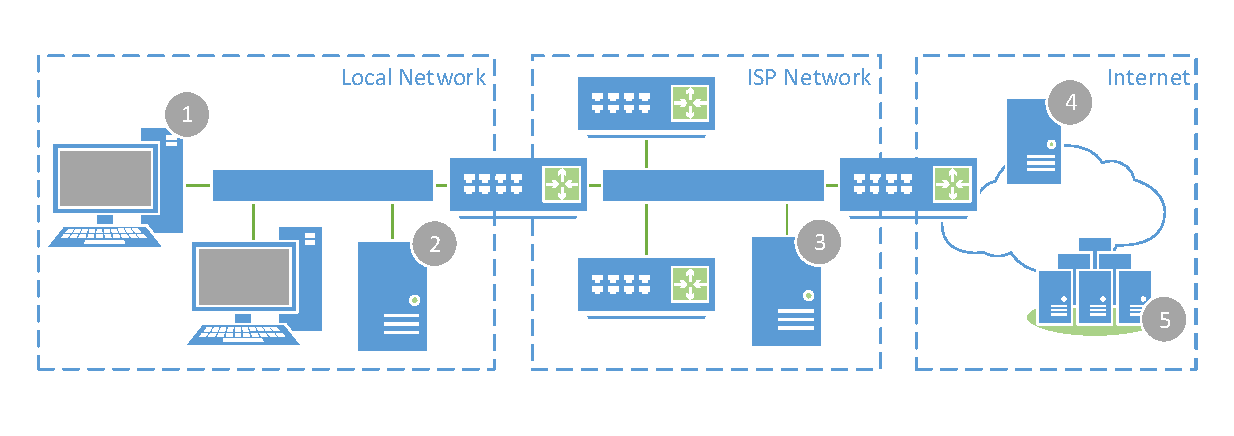
\includegraphics[width=\textwidth,trim={0 1cm 0 0.5cm},clip]{DNS_ResolverPosition}
    \caption{Zeigt die möglichen Positionen eines DNS-Resolvers. (1) Local-Loopback Resolver, (2) Local Recursive Resolver, (3) ISP Recursive Resolver, (4) Private Recursive Resolver, (5) Public Resolver}
    \label{img:dnsresolverposition}
\end{figure}
